\chapter{इलेक्ट्रोड बलगतिकी और विद्युतविश्लेषण}\label{ch:b3:electrode-kinetics}

प्लास्टिक की एक पट्टी पर रक्त की एक बूँद, पाँच सेकंड, एक संख्या: वह ग्लूकोस
मीटर, जिसे करोड़ों लोग दिन में कई बार उपयोग करते हैं, एक विद्युतरासायनिक
सेल है, और जो वह मापता है वह वोल्टता नहीं बल्कि धारा है। एक \omterm{def:b3:complex-kinetics:enzyme}{एंज़ाइम} ग्लूकोस का
ऑक्सीकरण करता है, एक घुला हुआ आयरन संकुल इलेक्ट्रॉनों को एक कार्बन
इलेक्ट्रोड तक ले जाता है, और बहने वाली धारा इस बात से तय होती है कि वह संकुल इलेक्ट्रोड तक
कितनी तेज़ी से विसरित होता है, अतः उसकी सांद्रता से। यह अध्याय समझाता है कि
इलेक्ट्रॉन किसी अंतरापृष्ठ को तेज़ी से या धीरे क्यों पार करते हैं (\omterm{thm:b3:electrode-kinetics:butler-volmer}{बटलर--वोल्मर समीकरण}),
द्रव्यमान परिवहन धारा को कैसे सीमित करता है, और \omterm{def:b3:electrode-kinetics:cv}{चक्रीय वोल्टामिति} तथा अन्य
विद्युतविश्लेषी विधियाँ धाराओं को सांद्रताओं, दर स्थिरांकों
और क्रियाविधियों में कैसे बदलती हैं।

\begin{recall}
प्रथम वर्ष के खंड ने इलेक्ट्रोड विभव, मानक विभव,
नेर्न्स्ट समीकरण, संदर्भ इलेक्ट्रोड और अर्ध-सेल परिभाषित किए। द्वितीय वर्ष के खंड ने
धारा--विभव वक्र, उनकी ऐनोडी और कैथोडी धाराओं के साथ,
कार्यकारी और प्रति-इलेक्ट्रोड, अधिविभव, तीव्र और मंद निकाय,
विसरण परत और सीमांत धारा; सक्रियता गुणांक और आयनिक
सामर्थ्य; अंशांकन वक्र, मानक-योग विधि और संसूचन
सीमा प्रस्तुत किए। \Cref{ch:b3:rate-theories} ने \omterm{def:b3:rate-theories:tst}{संक्रमण-अवस्था सिद्धांत} दिया। भौतिकी
से: विसरण के फ़िक के नियम, पॉयसाँ का समीकरण और संधारित्र।
\end{recall}

\begin{omfigure}
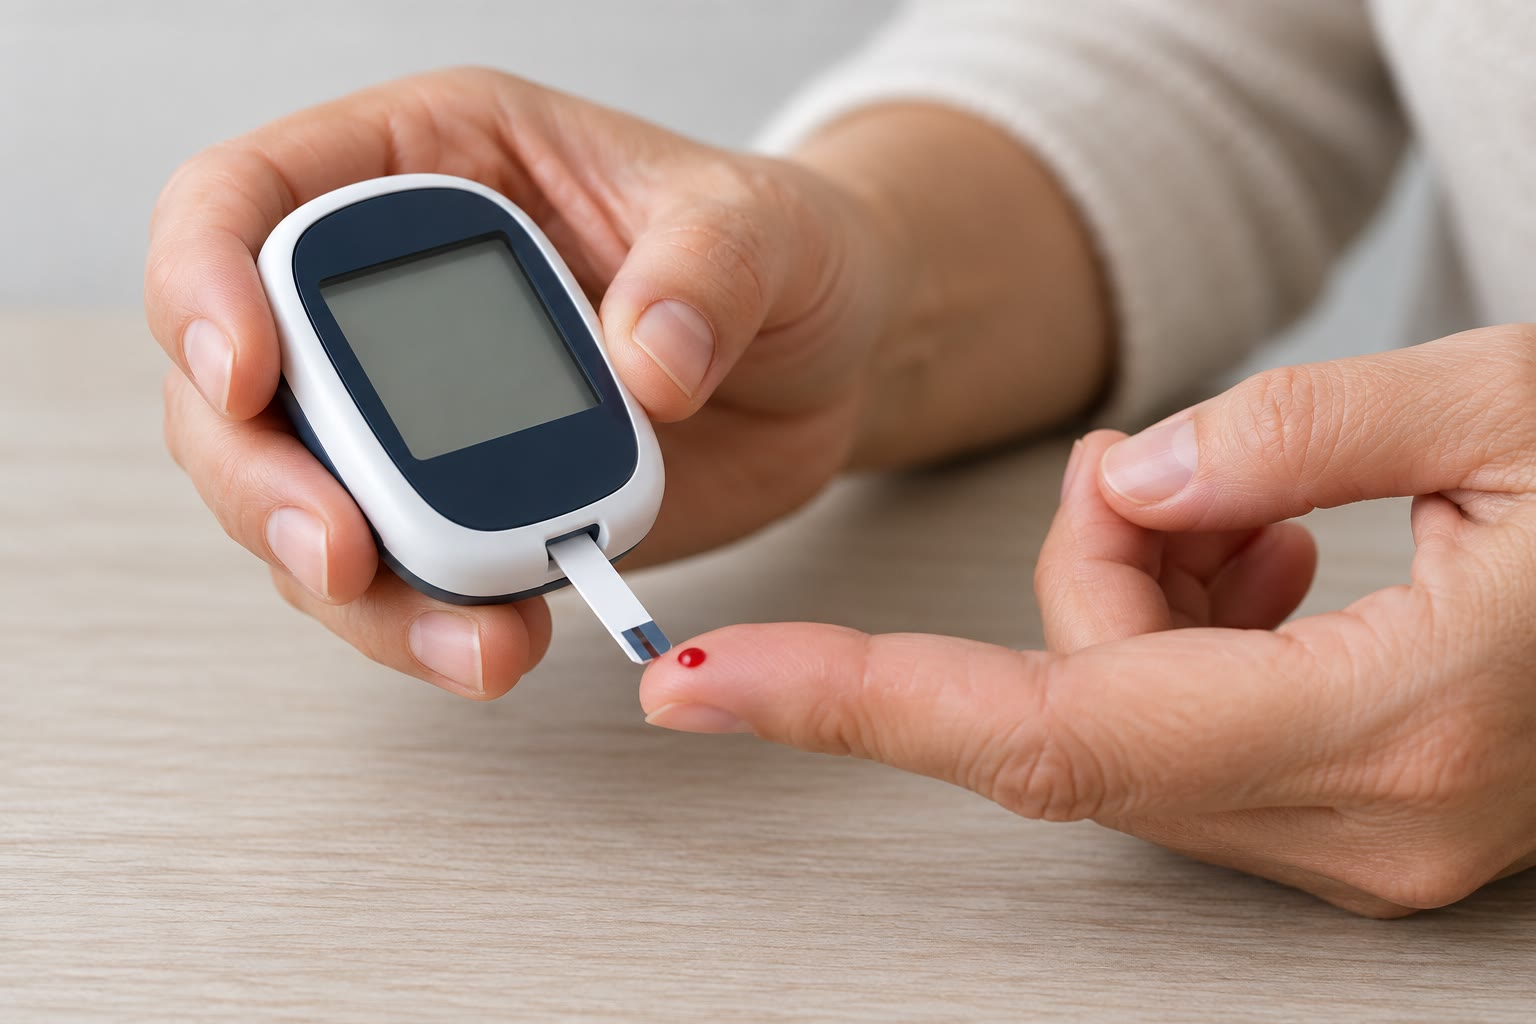
\includegraphics[width=0.6\linewidth]{images/book4/ai/b3-15-glucose-meter.jpg}

{\small एक रक्त-ग्लूकोस मीटर: पट्टी पर एक सूक्ष्म त्रि-इलेक्ट्रोड सेल होता है,
जिसमें एक \omterm{def:b3:complex-kinetics:enzyme}{एंज़ाइम} और एक रेडॉक्स मध्यस्थ होते हैं; मीटर एक विभव लगाता है और एक
धारा पढ़ता है।}
\end{omfigure}

\section{इलेक्ट्रोड--विलयन अंतरापृष्ठ}

किसी विद्युत-अपघट्य विलयन में डुबोई गई धातु पर एक पृष्ठीय आवेश होता है, और
विलयन उसका उत्तर एक समान और विपरीत आवेश से देता है, जो एक चिह्न के आयनों के
आधिक्य से बना होता है। आवेश की ये दो परतें आण्विक मोटाई का एक संधारित्र बनाती हैं।

\begin{definition}[वैद्युत द्विपरत]\label{def:b3:electrode-kinetics:double-layer}
\emph{वैद्युत द्विपरत}\index{वैद्युत द्विपरत} किसी इलेक्ट्रोड--विलयन अंतरापृष्ठ पर
आवेश की व्यवस्था है: धातु पर आवेश और विलयन में क्षतिपूरक
आयनिक आवेश। इसका संहत भाग,
\emph{हेल्महोल्ट्ज़ परत}\index{हेल्महोल्ट्ज़ परत}, पृष्ठ के संपर्क में स्थित आयनों और विलायक
अणुओं की परत है; इसकी \emph{विसरित परत}\index{विसरित परत}
उसके आगे का क्षेत्र है, जहाँ तापीय गति आधिक्य आयनों को
\emph{डिबाई लंबाई}\index{डिबाई लंबाई} $\kappa^{-1}$ की कोटि की दूरी पर फैला देती है।
\emph{द्विपरत संधारिता}\index{द्विपरत संधारिता} $C_{\mathrm{dl}}$ अंतरापृष्ठ के आर-पार प्रति वोल्ट
विभव, प्रति इकाई क्षेत्रफल संचित आवेश है।
\end{definition}

\begin{proposition}[डिबाई लंबाई]\label{prop:b3:electrode-kinetics:debye-length}
आयनिक सामर्थ्य $I$ (\unit{mol.m^{-3}} में) और आपेक्षिक परावैद्युतांक
$\varepsilon_r$ वाले विलयन में, इलेक्ट्रोड पर एक छोटा विभव $\varphi_0$ विलयन में
$\varphi = \varphi_0\eu^{-\kappa x}$ के रूप में क्षयित होता है, जहाँ
\[
  \kappa^{-1} = \sqrt{\frac{\varepsilon_r\varepsilon_0RT}{2F^2I}} .
\]
\end{proposition}

\begin{proof}
पॉयसाँ का समीकरण (भौतिकी से) विभव को आवेश घनत्व से संबंधित करता है:
$\dd^2\varphi/\dd x^2 = -\rho/\varepsilon_r\varepsilon_0$। प्रत्येक आयन विभव में \omterm{def:b3:partition-functions:boltzmann}{बोल्ट्समान वितरण} का पालन करता है:
$c_i = c_i^{\circ}\eu^{-z_iF\varphi/RT}$, अतः $\rho = F\sum_iz_ic_i^{\circ}\eu^{-z_iF\varphi/RT}$। $F\varphi \ll RT$ के लिए
$\eu^{-z_iF\varphi/RT} \approx 1 - z_iF\varphi/RT$; शून्य-कोटि पद विद्युत-उदासीनता से निरस्त हो जाते हैं,
और $\rho \approx -(F^2/RT)\sum_iz_i^2c_i^{\circ}\,\varphi = -(2F^2I/RT)\varphi$। अतः $\dd^2\varphi/\dd x^2 = \kappa^2\varphi$, जिसका
दूर शून्य होने वाला हल $\varphi_0\eu^{-\kappa x}$ है।
\end{proof}

\begin{example}[द्विपरत की मोटाई]\label{ex:b3:electrode-kinetics:debye}
% ledger: eps:H2O.25C, const:eps0, const:F, const:R
\qty{298.15}{K} पर जल में ($\varepsilon_r = 78.4$), 1:1 लवण के \qty{0.10}{mol/L} के साथ ($I = \qty{100}{mol.m^{-3}}$),
$\kappa^{-1} = \sqrt{78.4 \times \num{8.854e-12} \times 2479/(2 \times 96\,485^2 \times 100)} = \qty{0.96}{nm}$; \qty{1.0}{mmol/L} पर
यह दस गुना अधिक है। \omterm{def:b3:electrode-kinetics:transport}{सहायक विद्युत-अपघट्य} \omterm{def:b3:electrode-kinetics:double-layer}{विसरित परत} को कुछ
आण्विक व्यासों तक संपीडित कर देता है।
\end{example}

\omterm{def:b3:electrode-kinetics:double-layer}{विसरित परत} एक ऐसे संधारित्र की तरह व्यवहार करती है जिसकी प्लेटें $\kappa^{-1}$ दूर हैं: निम्न विभव पर
प्रति इकाई क्षेत्रफल इसकी संधारिता $\varepsilon_r\varepsilon_0\kappa$ है (गूई--चैपमैन
परिणाम; विभव पर इसकी निर्भरता स्वीकृत है)। संहत \omterm{def:b3:electrode-kinetics:double-layer}{हेल्महोल्ट्ज़ परत} के साथ
श्रेणी में यह मापित $C_{\mathrm{dl}}$ देती है, जो दसियों
माइक्रोफ़ैरड प्रति वर्ग सेंटीमीटर की कोटि की होती है (स्टर्न मॉडल)। जब भी विभव बदलता है, यह संधारित्र
आवेशित होता है: $v$ वोल्ट प्रति सेकंड की क्रमवीक्षण एक आवेशन धारा $C_{\mathrm{dl}}Av$ खींचती है, जो
कोई रसायन नहीं वहन करती और प्रत्येक वोल्टामितीय मापन में जुड़ जाती है।

\begin{omfigure}
\begin{tikzpicture}[font=\small, >=Stealth]
  \fill[black!25] (-1.0,0) rectangle (0,3.2);
  \node[rotate=90] at (-0.5,1.6) {धातु};
  \foreach \y in {0.3,0.8,...,2.9}{\node[font=\scriptsize] at (-0.15,\y) {$-$};}
  \foreach \y in {0.35,0.95,1.55,2.15,2.75}{\draw[omDef, fill=omDef!20] (0.3,\y) circle (0.18); \node[font=\scriptsize] at (0.3,\y) {$+$};}
  \draw[black!50, dashed] (0.55,0) -- (0.55,3.2);
  \node[font=\scriptsize, anchor=south, align=center] at (0.45,3.25) {हेल्महोल्ट्ज़\\ तल};
  \foreach \x/\y/\s in {1.1/0.6/+, 1.4/2.2/+, 1.9/1.3/+, 2.3/2.7/-, 2.6/0.5/+, 3.1/1.8/+, 3.5/0.9/-, 3.9/2.4/+, 4.4/1.4/-, 4.8/0.4/+, 5.1/2.8/-, 5.4/1.9/+}{
    \draw[black!60, fill=white] (\x,\y) circle (0.15); \node[font=\scriptsize] at (\x,\y) {$\s$};}
  \node[font=\scriptsize, anchor=south] at (3.2,3.25) {विसरित परत};
  \draw[->] (0,-2.1) -- (6.0,-2.1) node[anchor=north east] {$x$};
  \draw[->] (0,-2.1) -- (0,-0.3) node[anchor=east] {$|\varphi|$};
  \draw[omThm, thick] (0,-0.5) -- (0.55,-1.0) plot[domain=0.55:5.8, samples=40] (\x,{-2.1+1.1*exp(-(\x-0.55)/1.2)});
  \draw[black!40, dashed] (0.55,-2.1) -- (0.55,-0.4);
  \node[omThm, anchor=south west] at (1.3,-1.6) {$|\varphi(x)|$};
  \draw[<->, black!60] (0.55,-2.5) -- (1.75,-2.5) node[midway, below, font=\scriptsize] {$\sim\kappa^{-1}$};
\end{tikzpicture}

{\small \omterm{def:b3:electrode-kinetics:double-layer}{वैद्युत द्विपरत} (गूई--चैपमैन--स्टर्न मॉडल, व्यवस्थात्मक): एक
ऋणावेशित धातु, हेल्महोल्ट्ज़ तल पर धनायनों की एक संहत परत,
और एक \omterm{def:b3:electrode-kinetics:double-layer}{विसरित परत}, जहाँ कुछ डिबाई लंबाइयों तक धनायन ऋणायनों से अधिक होते हैं।
नीचे: विभव का परिमाण (ऋणात्मक, धातु के आवेश की तरह) संहत परत के आर-पार रैखिक रूप से,
फिर \omterm{def:b3:electrode-kinetics:double-layer}{विसरित परत} में चरघातांकी रूप से गिरता है।}
\end{omfigure}

\section{इलेक्ट्रॉन-स्थानांतरण बलगतिकी}

अपचयन $\mathrm{O} + n\,\mathrm{e}^- \to \mathrm{R}$ पर विचार कीजिए, जो विभव $E$ पर रखे गए एक इलेक्ट्रोड पर होता है,
जिसका स्थूल विलयन के लिए साम्य विभव $E_{\mathrm{eq}}$ होता।
अधिविभव $\eta = E - E_{\mathrm{eq}}$ है।

\begin{definition}[विनिमय धारा घनत्व, स्थानांतरण गुणांक, मानक दर स्थिरांक]\label{def:b3:electrode-kinetics:exchange}
साम्य पर ऐनोडी और कैथोडी धाराएँ बराबर और विपरीत होती हैं; प्रति इकाई क्षेत्रफल उनका
उभयनिष्ठ परिमाण \emph{विनिमय धारा
घनत्व}\index{विनिमय धारा घनत्व} $j_0$ है। \emph{स्थानांतरण गुणांक}
\index{स्थानांतरण गुणांक} $\alpha$ ($0 < \alpha < 1$) विद्युत ऊर्जा $nF\eta$ का वह
अंश है जो कैथोडी अभिक्रिया के अवरोध को घटाता है।
\emph{मानक दर स्थिरांक}\index{मानक दर स्थिरांक} $k^\circ$, औपचारिक विभव $E^{\circ\prime}$ पर
कैथोडी और ऐनोडी दर स्थिरांकों का उभयनिष्ठ मान है।
\end{definition}

\begin{theorem}[बटलर--वोल्मर समीकरण]\label{thm:b3:electrode-kinetics:butler-volmer}
यदि पृष्ठीय सांद्रताएँ स्थूल सांद्रताओं के बराबर हों (कोई द्रव्यमान-परिवहन
सीमा नहीं), तो ऐनोडी धाराओं को धनात्मक गिनते हुए, अधिविभव $\eta$ पर धारा घनत्व
है
\[
  j = j_0\bigl[\eu^{(1 - \alpha)f\eta} - \eu^{-\alpha f\eta}\bigr], \qquad f = \frac{nF}{RT}.
\]
यह \emph{बटलर--वोल्मर समीकरण}\index{बटलर--वोल्मर समीकरण} है।
\end{theorem}

\begin{proof}
\omterm{def:b3:rate-theories:tst}{संक्रमण-अवस्था सिद्धांत} से कैथोडी और ऐनोडी दर स्थिरांक
$k_{\mathrm c} = A\eu^{-\Delta G_{\mathrm c}^{\ddagger}/RT}$ और $k_{\mathrm a} = A\eu^{-\Delta G_{\mathrm a}^{\ddagger}/RT}$ हैं। इलेक्ट्रोड विभव को $\delta E$ से बदलने पर
अभिक्रिया $\mathrm{O} + n\,\mathrm{e}^- \to \mathrm{R}$ की गिब्स ऊर्जा $nF\,\delta E$ से बदल जाती है (धातु में इलेक्ट्रॉन
$-nF\,\delta E$ विद्युत ऊर्जा प्राप्त करते हैं)। प्रथम कोटि तक मान लीजिए कि इस परिवर्तन का एक
अंश $\alpha$ कैथोडी अवरोध में जाता है और शेष
ऐनोडी अवरोध में: $\Delta G_{\mathrm c}^{\ddagger} \to \Delta G_{\mathrm c}^{\ddagger} + \alpha nF\,\delta E$, $\Delta G_{\mathrm a}^{\ddagger} \to \Delta G_{\mathrm a}^{\ddagger} - (1 - \alpha)nF\,\delta E$। $\delta E$ को
साम्य विभव से मापने पर, जहाँ दोनों धाराएँ परिमाण में $j_0$
हैं, $j_{\mathrm c} = j_0\eu^{-\alpha f\eta}$ और $j_{\mathrm a} = j_0\eu^{(1 - \alpha)f\eta}$ मिलते हैं; नेट धारा उनका
अंतर है।
\end{proof}

\begin{corollary}[आवेश-स्थानांतरण प्रतिरोध]\label{cor:b3:electrode-kinetics:linear}
$|\eta| \ll RT/nF$ के लिए $j = j_0f\eta$: अंतरापृष्ठ एक प्रतिरोध
$R_{\mathrm{ct}} = RT/(nFi_0)$ की तरह व्यवहार करता है, जहाँ $i_0 = j_0A$।
\end{corollary}

\begin{proof}
दोनों चरघातांकियों का प्रथम कोटि तक प्रसार कीजिए: $j = j_0[(1 - \alpha)f\eta + \alpha f\eta] = j_0f\eta$; फिर
$\eta/i = 1/(fi_0)$।
\end{proof}

\begin{corollary}[टैफ़ेल समीकरण]\label{cor:b3:electrode-kinetics:tafel}
$\eta \ll -RT/nF$ (एक प्रबल कैथोडी अधिविभव) के लिए ऐनोडी पद
नगण्य होता है और
\[
  \eta = \frac{2.303\,RT}{\alpha nF}\bigl(\log j_0 - \log|j|\bigr):
\]
$\log|j|$, $\eta$ में रैखिक है, जिसका ढलान प्रति दशक $1/(\text{\qty{118}{mV}})$ है, \qty{298}{K} पर, $\alpha = 0.5$, $n =
1$ के लिए। यह \emph{टैफ़ेल समीकरण}\index{टैफ़ेल समीकरण} है।
\end{corollary}

\begin{proof}
$|j| = j_0\eu^{-\alpha f\eta}$, अतः $\ln|j| = \ln j_0 - \alpha f\eta$; दशमलव लघुगणकों में बदलिए।
\end{proof}

\begin{definition}[आवेश-स्थानांतरण प्रतिरोध, टैफ़ेल ढलान]\label{def:b3:electrode-kinetics:charge-transfer}
किसी इलेक्ट्रोड का \emph{आवेश-स्थानांतरण प्रतिरोध}\index{आवेश-स्थानांतरण प्रतिरोध}
$R_{\mathrm{ct}} = (\partial\eta/\partial i)_{\eta = 0}$ है। \emph{टैफ़ेल ढलान}\index{टैफ़ेल ढलान}
टैफ़ेल क्षेत्र में धारा के प्रति दशक अधिविभव का परिवर्तन है,
$2.303\,RT/\alpha nF$।
\end{definition}

\begin{omfigure}
\begin{tikzpicture}
\begin{axis}[name=bv, omcv, width=0.47\linewidth, height=5.4cm, xmin=-300, xmax=300, ymin=-40, ymax=40,
  xlabel={$\eta$ / mV}, ylabel={$j/j_0$},
  legend style={font=\scriptsize, draw=none, at={(0.03,0.97)}, anchor=north west}, legend cell align=left]
\addplot[omDef, thick] table[x=eta_mV, y=a3] {figdata/out/bachelor-3-butler-volmer.dat};
\addplot[black, thick] table[x=eta_mV, y=a5] {figdata/out/bachelor-3-butler-volmer.dat};
\addplot[omThm, thick] table[x=eta_mV, y=a7] {figdata/out/bachelor-3-butler-volmer.dat};
\legend{$\alpha = 0.3$, $\alpha = 0.5$, $\alpha = 0.7$}
\draw[black!30] (axis cs:-300,0) -- (axis cs:300,0) (axis cs:0,-40) -- (axis cs:0,40);
\end{axis}
\begin{axis}[at={(bv.east)}, anchor=west, xshift=1.2cm, omcv, width=0.47\linewidth, height=5.4cm,
  xmin=-300, xmax=300, ymin=-1.5, ymax=4, xlabel={$\eta$ / mV}, ylabel={$\log|j/j_0|$},
  unbounded coords=jump]
\addplot[omDef, thick] table[x=eta_mV, y=l3] {figdata/out/bachelor-3-butler-volmer.dat};
\addplot[black, thick] table[x=eta_mV, y=l5] {figdata/out/bachelor-3-butler-volmer.dat};
\addplot[omThm, thick] table[x=eta_mV, y=l7] {figdata/out/bachelor-3-butler-volmer.dat};
\draw[black!40, dashed] (axis cs:-300,2.54) -- (axis cs:0,0);
\draw[black!50] (axis cs:-200,1.85) -- (axis cs:-120,3.3) node[anchor=south, font=\scriptsize, inner sep=1pt] {ढलान $1/(\qty{118}{mV})$};
\end{axis}
\end{tikzpicture}

{\small तीन \omterm{def:b3:electrode-kinetics:exchange}{स्थानांतरण गुणांकों} के लिए \omterm{thm:b3:electrode-kinetics:butler-volmer}{बटलर--वोल्मर समीकरण} ($n = 1$, \qty{298}{K})।
बाएँ: साम्य के निकट धारा $\eta$ में रैखिक है (\omterm{def:b3:electrode-kinetics:charge-transfer}{आवेश-स्थानांतरण
प्रतिरोध}) और उससे आगे चरघातांकी; $\alpha$ इसे असममित बनाता है।
दाएँ: टैफ़ेल आलेख, जिसकी सीधी शाखाएँ $\log|j/j_0| = 0$ तक बहिर्वेशित होती हैं,
$\eta = 0$ पर; धराशायी रेखा $\alpha = 0.5$ के लिए कैथोडी टैफ़ेल रेखा है।}
\end{omfigure}

\begin{method}[एक टैफ़ेल विश्लेषण]\label{met:b3:electrode-kinetics:tafel-analysis}
\begin{enumerate}
  \item विलोडित विलयन में, सीमांत धारा से काफ़ी नीचे (या द्रव्यमान परिवहन के लिए संशोधन करके),
        $\eta$ के विरुद्ध स्थायी धारा अभिलिखित कीजिए।
  \item $\log|i|$ को $\eta$ के विरुद्ध आलेखित कीजिए; लगभग \qty{100}{mV} से आगे की रैखिक शाखा समंजित कीजिए।
  \item ढलान $\alpha$ देता है (या ऐनोडी शाखा पर $1 - \alpha$); $\eta = 0$ पर अंतःखंड
        $\log i_0$ देता है।
  \item जाँच: $\eta = 0$ के निकट, $i$ का $\eta$ के विरुद्ध ढलान $1/R_{\mathrm{ct}} = nFi_0/RT$ है।
\end{enumerate}
\end{method}

द्वितीय वर्ष के खंड के तीव्र और मंद निकाय इस चित्र के दो छोर हैं: तीव्र निकाय का
$j_0$ बड़ा होता है और उसका धारा--विभव वक्र साम्य विभव पर तेज़ी से
उठता है; मंद निकाय को कोई धारा बहने से पहले बड़े अधिविभव की आवश्यकता होती है।
एक ही अभिक्रिया का \omterm{def:b3:electrode-kinetics:exchange}{विनिमय धारा घनत्व} एक इलेक्ट्रोड पदार्थ से दूसरे तक परिमाण की अनेक
कोटियों में बदलता है: हाइड्रोजन का निकास प्लैटिनम पर तीव्र और पारे पर अत्यंत मंद है।

\section{द्रव्यमान परिवहन}

\begin{definition}[द्रव्यमान परिवहन की विधाएँ]\label{def:b3:electrode-kinetics:transport}
स्पीशीज़ किसी इलेक्ट्रोड तक \emph{अभिगमन}\index{अभिगमन} द्वारा, अर्थात् विद्युत क्षेत्र में आयनों
की गति द्वारा; विसरण द्वारा, सांद्रता प्रवणताओं की दिशा में; और
\emph{संवहन}\index{संवहन} द्वारा, अर्थात् पूरे विलयन की गति द्वारा
(विलोडन, घूर्णन, प्रवाह), पहुँचती हैं। \emph{सहायक विद्युत-अपघट्य}\index{सहायक विद्युत-अपघट्य}
बड़े आधिक्य में मिलाया गया एक अक्रिय लवण है, जो विलयन से होकर लगभग सारी
धारा वहन करता है, ताकि विद्युत-सक्रिय स्पीशीज़ केवल विसरण और संवहन द्वारा
गति करे।
\end{definition}

\begin{definition}[काल-ऐम्पियरमिति]\label{def:b3:electrode-kinetics:chronoamperometry}
\emph{काल-ऐम्पियरमिति}\index{काल-ऐम्पियरमिति} इलेक्ट्रोड विभव के एक सोपान के बाद
समय के विरुद्ध धारा अभिलिखित करती है।
\end{definition}

\begin{theorem}[कॉटरेल समीकरण]\label{thm:b3:electrode-kinetics:cottrell}
$t = 0$ पर एक ऐसे मान तक विभव-सोपान के बाद, जहाँ विद्युत-सक्रिय स्पीशीज़
क्षेत्रफल $A$ वाले समतल इलेक्ट्रोड तक पहुँचते ही उपभुक्त हो जाती है, \omterm{def:b3:electrode-kinetics:transport}{सहायक
विद्युत-अपघट्य} वाले शांत विलयन में धारा है
\[
  i = nFAc^*\sqrt{\frac{D}{\pi t}},
\]
जहाँ $c^*$ स्थूल सांद्रता है और $D$ विसरण गुणांक। यह
\emph{कॉटरेल समीकरण}\index{कॉटरेल समीकरण} है।
\end{theorem}

\begin{proof}
सांद्रता फ़िक के द्वितीय नियम $\partial c/\partial t = D\,\partial^2c/\partial x^2$ का पालन करती है, जहाँ $c(x, 0) = c^*$,
$c(0, t) = 0$ ($t > 0$ के लिए) और दूर $c \to c^*$। फलन $c = c^*\operatorname{erf}(x/2\sqrt{Dt})$, जहाँ
$\operatorname{erf}u = \frac{2}{\sqrt\pi}\int_0^u\eu^{-s^2}\dd s$, इन शर्तों को संतुष्ट करता है: $\operatorname{erf}0 = 0$, $\operatorname{erf}u \to 1$ जब $u \to \infty$
($t \to 0$ पर प्रत्येक $x > 0$ के लिए, और दूर)। $u = x/2\sqrt{Dt}$ लेने पर,
$\partial c/\partial t = c^*\frac{2}{\sqrt\pi}\eu^{-u^2}\partial u/\partial t = -c^*\frac{2}{\sqrt\pi}\eu^{-u^2}\frac{u}{2t}$ और $\partial^2c/\partial x^2 = c^*\frac{2}{\sqrt\pi}(-2u)\eu^{-u^2}\frac{1}{4Dt}$: फ़िक के नियम की
दोनों भुजाएँ मेल खाती हैं। धारा पृष्ठ पर फ़्लक्स है: $i =
nFAD(\partial c/\partial x)_{x = 0} = nFADc^*\frac{2}{\sqrt\pi}\frac{1}{2\sqrt{Dt}} = nFAc^*\sqrt{D/\pi t}$। (हल की अद्वितीयता
स्वीकृत है।)
\end{proof}

\begin{omfigure}
\begin{tikzpicture}
\begin{axis}[name=pr, width=0.47\linewidth, height=5.2cm, xmin=0, xmax=600, ymin=0, ymax=1.08,
  axis lines=left, xlabel={$x$ / \unit{\micro m}}, ylabel={$c/c^*$},
  tick label style={font=\small}, label style={font=\small},
  legend style={font=\scriptsize, draw=none, at={(0.97,0.03)}, anchor=south east}, legend cell align=left]
\addplot[omDef, thick] table[x=x_um, y=t1] {figdata/out/bachelor-3-cottrell-profiles.dat};
\addplot[black!60, thick] table[x=x_um, y=t2] {figdata/out/bachelor-3-cottrell-profiles.dat};
\addplot[omThm, thick] table[x=x_um, y=t3] {figdata/out/bachelor-3-cottrell-profiles.dat};
\addplot[black, thick, dashed] table[x=x_um, y=t4] {figdata/out/bachelor-3-cottrell-profiles.dat};
\legend{\qty{0.1}{s}, \qty{1}{s}, \qty{4}{s}, \qty{16}{s}}
\end{axis}
\begin{axis}[at={(pr.east)}, anchor=west, xshift=1.3cm, width=0.47\linewidth, height=5.2cm,
  xmin=0, xmax=3.3, ymin=0, ymax=40, axis lines=left, xlabel={$t^{-1/2}$ / \unit{s^{-1/2}}},
  ylabel={$i$ / \unit{\micro A}}, tick label style={font=\small}, label style={font=\small}]
\addplot[omDef, very thick] table[x=tm12, y=i_uA] {figdata/out/bachelor-3-cottrell-current.dat};
\end{axis}
\end{tikzpicture}

{\small \omterm{def:b3:electrode-kinetics:chronoamperometry}{काल-ऐम्पियरमिति} (मॉडल: $D = \qty{1.0e-5}{cm^2.s^{-1}}$, $c^* = \qty{1.0}{mM}$, \qty{3}{mm} की
डिस्क)। बाएँ: अवक्षय परत $\sqrt{Dt}$ के अनुसार बढ़ती है, \qty{0.1}{s} के बाद लगभग \qty{30}{\micro m}
और \qty{16}{s} के बाद \qty{350}{\micro m}। दाएँ: कॉटरेल धारा
$t^{-1/2}$ के समानुपाती है; इसका ढलान $D$ देता है।}
\end{omfigure}

विलोडित विलयन या घूर्णी डिस्क इलेक्ट्रोड विसरण परत को एक
स्थिर मोटाई $\delta$ पर रखता है: धारा द्वितीय वर्ष के खंड के स्थायी सीमांत मान $nFADc^*/\delta$
तक पहुँचती है। घूर्णी डिस्क के लिए $\delta$ घूर्णन दर के वर्गमूल के व्युत्क्रम के अनुसार
घटता है (लेविच, स्वीकृत), जिससे सीमांत धारा
$\sqrt\omega$ के समानुपाती हो जाती है।

\section{चक्रीय वोल्टामिति}

\begin{definition}[चक्रीय वोल्टामिति]\label{def:b3:electrode-kinetics:cv}
\emph{चक्रीय वोल्टामिति}\index{चक्रीय वोल्टामिति} एक स्थिर कार्यकारी इलेक्ट्रोड के विभव को
समय के साथ रैखिकतः दो सीमाओं के बीच और वापस, क्रमवीक्षण दर $v$ पर, एक शांत विलयन में
घुमाती है, और धारा अभिलिखित करती है। विभव के विरुद्ध धारा का आलेख
\emph{वोल्टामोग्राम}\index{वोल्टामोग्राम} है; प्रत्येक तरंग की एक
\emph{शिखर धारा}\index{शिखर धारा} $i_{\mathrm p}$ होती है, उसके \emph{शिखर विभव}\index{शिखर विभव}
$E_{\mathrm p}$ पर।
\end{definition}

शिखर दो प्रतिस्पर्धी प्रभावों से उत्पन्न होता है। जैसे-जैसे विभव $E^{\circ\prime}$ से आगे बढ़ता है,
अभिकारक की पृष्ठीय सांद्रता गिरती है (नेर्न्स्ट समीकरण, तीव्र
निकाय के लिए) और धारा बढ़ती है; परंतु अवक्षयित परत समय के साथ मोटी होती है और
फ़्लक्स गिरता है। वापसी क्रमवीक्षण पर उत्पाद, जो अब भी इलेक्ट्रोड के निकट है, फिर से
रूपांतरित हो जाता है।

\begin{definition}[उत्क्रमणीयता]\label{def:b3:electrode-kinetics:reversibility}
विमाहीन दर प्राचल $\Lambda = k^\circ/\sqrt{DnFv/RT}$ के साथ, जो
इलेक्ट्रॉन-स्थानांतरण दर की तुलना क्रमवीक्षण द्वारा आरोपित विसरण दर से करता है, कोई
युग्म \emph{विद्युतरासायनिकतः उत्क्रमणीय}\index{विद्युतरासायनिकतः उत्क्रमणीय निकाय}
है यदि $\Lambda > 15$ (उसकी पृष्ठीय सांद्रताएँ हर समय नेर्न्स्ट समीकरण का
पालन करती हैं), \emph{अर्ध-उत्क्रमणीय}\index{अर्ध-उत्क्रमणीय निकाय} यदि $15 >
\Lambda > 10^{-2(1 + \alpha)}$, और इससे नीचे \emph{विद्युतरासायनिकतः अनुत्क्रमणीय}\index{विद्युतरासायनिकतः अनुत्क्रमणीय निकाय}
है।
\end{definition}

\begin{remark}
द्वितीय वर्ष के खंड के तीव्र और मंद निकाय इस
वर्गीकरण के अनुरूप हैं, परंतु एक अंतर के साथ: यहाँ उत्क्रमणीयता क्रमवीक्षण
दर पर निर्भर करती है। वही युग्म \qty{10}{mV/s} पर उत्क्रमणीय और
\qty{10}{V/s} पर \omterm{def:b3:electrode-kinetics:reversibility}{अर्ध-उत्क्रमणीय} हो सकता है, क्योंकि तेज़ क्रमवीक्षण इलेक्ट्रॉन स्थानांतरण के लिए कम समय छोड़ता है।
\end{remark}

\begin{proposition}[रैंडल्स--शेवचीक समीकरण]\label{prop:b3:electrode-kinetics:randles-sevcik}
\qty{298}{K} पर समतल इलेक्ट्रोड पर एक उत्क्रमणीय तरंग के लिए,
\[
  i_{\mathrm p} = 0.4463\,nFAc^*\sqrt{\frac{nFvD}{RT}},
\]
अतः $i_{\mathrm p} \propto \sqrt v$। यह \emph{रैंडल्स--शेवचीक समीकरण}\index{रैंडल्स--शेवचीक समीकरण} है।
\end{proposition}

\begin{proof}[आंशिक उपपत्ति]
चरों $\xi = x\sqrt{nFv/(RTD)}$ और $\theta = nFvt/RT$ में (विभव क्रमवीक्षण,
$RT/nF$ की इकाइयों में), पृष्ठ पर नेर्न्स्ट शर्त सहित फ़िक के नियम में आरंभिक विभव के अतिरिक्त
कोई प्राचल नहीं होता: विमाहीन फ़्लक्स एक
सार्वत्रिक फलन $\chi(\theta)$ है। भौतिक इकाइयों में लौटने पर, $i = nFAc^*\sqrt{nFvD/RT}\,\chi(\theta)$: हर
धारा, शिखर सहित, $\sqrt v$ के अनुसार बदलती है।
$\chi$ के अधिकतम का मान 0.4463 एक संख्यात्मक हल से आता है (स्वीकृत; चित्र का अनुकरण
इसे 0.1\,\% तक पुनरुत्पन्न करता है)।
\end{proof}

\begin{proposition}[शिखर पृथक्करण]\label{prop:b3:electrode-kinetics:delta-ep}
उत्क्रमणीय तरंग के लिए कैथोडी और ऐनोडी शिखर लगभग \qty{28.5}{mV}$/n$ की दूरी पर,
$E^{\circ\prime}$ के दोनों ओर, स्थित होते हैं (\qty{298}{K} पर, तरंग से बहुत आगे के व्युत्क्रमण विभव के लिए):
$\Delta E_{\mathrm p} \approx 57/n$ \unit{mV}, क्रमवीक्षण दर से स्वतंत्र, और $E_{1/2} = (E_{\mathrm{pc}} + E_{\mathrm{pa}})/2 =
E^{\circ\prime}$, जब दोनों स्पीशीज़ के विसरण गुणांक बराबर हों।
\end{proposition}

\begin{proof}[आंशिक उपपत्ति]
पिछली उपपत्ति के विमाहीन रूप में शिखर $\theta$ के एक नियत
मान पर आता है, अर्थात् $E^{\circ\prime}$ के सापेक्ष एक नियत विभव पर, $v$ चाहे जो हो;
O और R के बीच नेर्न्स्ट शर्त की सममिति ऐनोडी शिखर को
सममित रूप से रखती है। संख्यात्मक मान स्वीकृत है; अनुकरण
$\pm\qty{28.5}{mV}$, $\Delta E_{\mathrm p} = \qty{57.7}{mV}$ देता है।
\end{proof}

\begin{omfigure}
\begin{tikzpicture}
\begin{axis}[name=cv, omcv, width=0.62\linewidth, height=6.4cm, xmin=-320, xmax=320, ymin=-30, ymax=22,
  xlabel={$E - E^{\circ\prime}$ / mV}, ylabel={$i$ / \unit{\micro A}},
  legend style={font=\scriptsize, draw=none, fill=white, fill opacity=0.85, text opacity=1,
  at={(0.01,0.99)}, anchor=north west}, legend cell align=left]
\addplot[black!40, thin] table[x=E_mV, y=i_uA] {figdata/out/bachelor-3-cyclic-voltammetry-v25.dat};
\addplot[omDef!60, thin] table[x=E_mV, y=i_uA] {figdata/out/bachelor-3-cyclic-voltammetry-v50.dat};
\addplot[omDef, thick] table[x=E_mV, y=i_uA] {figdata/out/bachelor-3-cyclic-voltammetry-v100.dat};
\addplot[black, thick] table[x=E_mV, y=i_uA] {figdata/out/bachelor-3-cyclic-voltammetry-v200.dat};
\addplot[omThm, thick, dashed] table[x=E_mV, y=i_uA] {figdata/out/bachelor-3-cyclic-voltammetry-quasi.dat};
\legend{\qty{25}{mV/s}, \qty{50}{mV/s}, \qty{100}{mV/s}, \qty{200}{mV/s}, {अर्ध-उत्क्रमणीय, \qty{100}{mV/s}}}
\end{axis}
\begin{axis}[at={(cv.east)}, anchor=west, xshift=1.3cm, width=0.32\linewidth, height=5.0cm,
  xmin=0, xmax=0.5, ymin=0, ymax=30, axis lines=left, xlabel={$\sqrt v$ / \unit{(V/s)^{1/2}}},
  ylabel={$|i_{\mathrm{pc}}|$ / \unit{\micro A}}, tick label style={font=\small}, label style={font=\small}]
\addplot[only marks, mark=*, omDef] table[x=sqrtv, y=ip_uA] {figdata/out/bachelor-3-cyclic-voltammetry-ip.dat};
\addplot[black, domain=0:0.5] {60.06*x};
\end{axis}
\end{tikzpicture}

{\small एक अपचयन के लिए परिमित अंतरों द्वारा अनुकरित चक्रीय \omterm{def:b3:electrode-kinetics:cv}{वोल्टामोग्राम}
(मॉडल: \qty{1.0}{mM}, $D = \qty{1.0e-5}{cm^2.s^{-1}}$, \qty{3}{mm} डिस्क, $n = 1$; ऐनोडी धारा
धनात्मक)। चार क्रमवीक्षण दरों पर उत्क्रमणीय तरंगें: शिखर \qty{57.7}{mV} दूर रहते हैं,
$E^{\circ\prime}$ पर केंद्रित, और \omterm{def:b3:electrode-kinetics:cv}{शिखर धारा} $\sqrt v$ के अनुसार बढ़ती है (दाएँ, रेखा
\omterm{prop:b3:electrode-kinetics:randles-sevcik}{रैंडल्स--शेवचीक समीकरण} है)। धराशायी: एक \omterm{def:b3:electrode-kinetics:reversibility}{अर्ध-उत्क्रमणीय} युग्म ($k^\circ = \qty{2e-3}{cm.s^{-1}}$),
\qty{100}{mV/s} पर, जिसके शिखर \qty{162}{mV} दूर और नीचे हैं।}
\end{omfigure}

\begin{method}[वोल्टामोग्राम का निदान]\label{met:b3:electrode-kinetics:cv-diagnosis}
\begin{enumerate}
  \item उत्क्रमणीय: हर क्रमवीक्षण दर पर $\Delta E_{\mathrm p} \approx 57/n$ \unit{mV}, $|i_{\mathrm{pa}}/i_{\mathrm{pc}}| = 1$, $i_{\mathrm p} \propto \sqrt v$;
        $E_{1/2}$ से $E^{\circ\prime}$ मिलता है।
  \item \omterm{def:b3:electrode-kinetics:reversibility}{अर्ध-उत्क्रमणीय}: $\Delta E_{\mathrm p}$ क्रमवीक्षण दर के साथ बढ़ता है; इसका मान $k^\circ$ देता है।
  \item अनुत्क्रमणीय: कोई वापसी शिखर नहीं; \omterm{def:b3:electrode-kinetics:cv}{शिखर विभव} क्रमवीक्षण दर के प्रति दशक $30/\alpha n$ \unit{mV}
        खिसकता है।
  \item एक अनुवर्ती रासायनिक चरण (EC क्रियाविधि): धीमे क्रमवीक्षणों पर वापसी शिखर
        अग्र शिखर से छोटा होता है और तेज़ क्रमवीक्षणों पर, जो रसायन से आगे निकल जाते हैं,
        पुनः बहाल हो जाता है।
  \item अधिशोषित स्पीशीज़: $i_{\mathrm p} \propto v$, $\sqrt v$ नहीं।
\end{enumerate}
\end{method}

अजलीय विलायकों में, जहाँ संदर्भ इलेक्ट्रोड विचलित होते हैं, विभवों को प्रयोग के अंत में
मिलाए गए एक आंतरिक मानक के सापेक्ष व्यक्त किया जाता है:
फ़ेरोसीनियम/फ़ेरोसीन युग्म, जो अधिकांश कार्बनिक विलायकों में तीव्र और सुव्यवहारी है।

\begin{method}[त्रि-इलेक्ट्रोड मापन की व्यवस्था]\label{met:b3:electrode-kinetics:three-electrode}
\begin{enumerate}
  \item कार्यकारी इलेक्ट्रोड (काँचाभ कार्बन, प्लैटिनम, स्वर्ण) ताज़ा पॉलिश किया हुआ;
        अधिक क्षेत्रफल का प्रति-इलेक्ट्रोड (प्लैटिनम तार); संदर्भ इलेक्ट्रोड
        (Ag/AgCl, या आंतरिक मानक के साथ रजत तार) कार्यकारी इलेक्ट्रोड
        के निकट।
  \item विश्लेष्य का विलयन (लगभग 1 \unit{mM}), \omterm{def:b3:electrode-kinetics:transport}{सहायक विद्युत-अपघट्य} के \qty{0.1}{mol/L}
        के साथ, आर्गन से विगैसित (घुली हुई ऑक्सीजन
        मध्यम ऋणात्मक विभवों पर अपचयित होती है और अपनी तरंगें जोड़ देती)।
  \item विभवस्थापी कार्यकारी और संदर्भ इलेक्ट्रोडों के बीच विभव को स्थिर रखता है
        और धारा को कार्यकारी और प्रति-इलेक्ट्रोडों के बीच
        प्रवाहित करता है; संदर्भ इलेक्ट्रोड से कोई धारा नहीं बहती।
\end{enumerate}
\end{method}

\begin{omfigure}
\begin{tikzpicture}[font=\small, >=Stealth]
  \begin{scope}[scale=1.5]
    \pic[transform shape] at (0,0) {beaker={0.7}{omWater!60}};
    \pic[transform shape] at (-0.45,0.35) {electrode={black!70}};
    \pic[transform shape] at (0,0.35) {electrode={black!20}};
    \pic[transform shape] at (0.45,0.35) {probe};
  \end{scope}
  \draw[thick] (-1.6,6.0) rectangle (1.6,7.2);
  \node at (0,6.6) {विभवस्थापी};
  \draw[thick, omDef] (-0.675,4.35) |- (-1.0,5.2) -- (-1.0,6.0);
  \draw[thick, black!60] (0,4.35) -- (0,6.0);
  \draw[thick, omThm] (0.675,5.18) |- (1.0,5.5) -- (1.0,6.0);
  \node[omDef, anchor=east, align=right, font=\scriptsize] at (-1.1,5.2) {कार्यकारी};
  \node[black!70, rotate=90, anchor=north, font=\scriptsize, inner sep=1pt] at (0.06,5.35) {प्रति};
  \node[omThm, anchor=west, align=left, font=\scriptsize] at (1.1,5.2) {संदर्भ};
\end{tikzpicture}

{\small एक त्रि-इलेक्ट्रोड सेल। विभवस्थापी कार्यकारी इलेक्ट्रोड के विभव को
संदर्भ इलेक्ट्रोड के सापेक्ष नियंत्रित करता है, जिससे कोई धारा नहीं बहती,
और धारा को प्रति-इलेक्ट्रोड से होकर प्रवाहित करता है।}
\end{omfigure}

\section{विद्युतविश्लेषी विधियाँ}

\begin{definition}[ऐम्पियरमिति, जैवसंवेदक]\label{def:b3:electrode-kinetics:amperometry}
\emph{ऐम्पियरमिति}\index{ऐम्पियरमिति} एक नियत विभव पर धारा मापती है, जो
अभिक्रिया करने वाली स्पीशीज़ की सांद्रता के समानुपाती होती है।
\emph{जैवसंवेदक}\index{जैवसंवेदक} एक जैविक अभिज्ञान तत्व (एक
\omterm{def:b3:complex-kinetics:enzyme}{एंज़ाइम}, एक प्रतिपिंड) को एक पारक्रमित्र से, यहाँ एक इलेक्ट्रोड से, जोड़ता है।
\end{definition}

\emergencystretch=3em ग्लूकोस पट्टी में ग्लूकोस ऑक्सीडेज़ ग्लूकोस को ग्लूकोनोलैक्टोन में ऑक्सीकृत करता है और
एक मध्यस्थ, हेक्सासायनोफ़ेरेट(III), द्वारा पुनर्जनित होता है, जो अपचयित हो जाता है;
इलेक्ट्रोड पर, जिसे ऐसे विभव पर रखा जाता है जहाँ हेक्सासायनोफ़ेरेट(II) ऑक्सीकृत होता है,
धारा बने हुए मध्यस्थ को मापती है, प्रति ग्लूकोस दो:
\[
  \ce{C6H12O6 + 2 [Fe(CN)6]^3- -> C6H10O6 + 2 [Fe(CN)6]^4- + 2 H+} .
\]

\begin{definition}[ऐनोडी विलोपन वोल्टामिति]\label{def:b3:electrode-kinetics:stripping}
\emph{ऐनोडी विलोपन वोल्टामिति}\index{ऐनोडी विलोपन वोल्टामिति}
किसी धातु के आयनों को एक नियत समय तक, एक नियत विभव पर, इलेक्ट्रोड पर अपचयित करके
उस धातु का पूर्वसांद्रण करती है, फिर विभव का ऐनोडी क्रमवीक्षण करती है और उसके
पुनःऑक्सीकरण की \omterm{def:b3:electrode-kinetics:cv}{शिखर धारा} मापती है, जो विलयन में सांद्रता के
समानुपाती होती है।
\end{definition}

पूर्वसांद्रण इस विधि को पेयजल में सीसे या
कैडमियम के अंशों के लिए, माइक्रोग्राम प्रति लीटर के स्तर पर, पर्याप्त सुग्राही बना देता है। चूँकि
सुग्राहिता आधात्री पर निर्भर करती है, इसका अंशांकन स्वयं नमूने में,
मानक योगों द्वारा, किया जाता है।

\begin{method}[विलोपन के साथ मानक योग]\label{met:b3:electrode-kinetics:standard-addition}
\begin{enumerate}
  \item नमूने का विलोपन शिखर अभिलिखित कीजिए, फिर किसी मानक के तीन या अधिक
        योगों के बाद, जिनमें से प्रत्येक सांद्रता को एक ज्ञात मात्रा से बढ़ाता है
        (छोटे आयतन, ताकि तनुकरण नगण्य हो या उसका संशोधन किया जाए)।
  \item मिलाई गई सांद्रता के विरुद्ध शिखर ऊँचाई समंजित कीजिए: एक सीधी रेखा।
  \item सांद्रता अक्ष पर इसका अंतःखंड नमूने की सांद्रता का ऋण है;
        रेखा की मानक त्रुटियों का परिणाम तक संचरण कीजिए।
\end{enumerate}
\end{method}

\begin{omfigure}
\begin{tikzpicture}
\begin{axis}[name=sp, omcv, width=0.47\linewidth, height=5.2cm, xmin=-600, xmax=-300, ymin=0, ymax=2.4,
  xlabel={$E$ / mV}, ylabel={$i$ / \unit{\micro A}}]
\addplot[black, thick] table[x=E_mV, y=s0] {figdata/out/bachelor-3-standard-addition-peaks.dat};
\addplot[omDef!50, thick] table[x=E_mV, y=s1] {figdata/out/bachelor-3-standard-addition-peaks.dat};
\addplot[omDef!80, thick] table[x=E_mV, y=s2] {figdata/out/bachelor-3-standard-addition-peaks.dat};
\addplot[omDef, thick] table[x=E_mV, y=s3] {figdata/out/bachelor-3-standard-addition-peaks.dat};
\end{axis}
\begin{axis}[at={(sp.east)}, anchor=west, xshift=1.3cm, width=0.47\linewidth, height=5.2cm,
  xmin=-6, xmax=16, ymin=0, ymax=2.3, axis x line=middle, axis y line=left,
  xlabel={मिलाया गया Pb / \unit{\micro g.L^{-1}}}, ylabel={शिखर ऊँचाई / \unit{\micro A}},
  tick label style={font=\small}, label style={font=\small},
  xlabel style={at={(0.5,-0.18)}, anchor=north}]
\addplot[black, thin] table[x=added, y=h] {figdata/out/bachelor-3-standard-addition-line.dat};
\addplot[only marks, mark=*, omDef] table[x=added, y=h] {figdata/out/bachelor-3-standard-addition-points.dat};
\node[font=\scriptsize, anchor=south] at (axis cs:-4.26,0.05) {$-c_0$};
\end{axis}
\end{tikzpicture}

{\small तीन मानक योगों के साथ सीसे का ऐनोडी विलोपन (\cref{exo:b3:electrode-kinetics:9}
के आँकड़े)। बाएँ: प्रत्येक योग के साथ विलोपन शिखर
बढ़ते हैं। दाएँ: मिलाई गई सांद्रता के विरुद्ध शिखर ऊँचाई की न्यूनतम-वर्ग रेखा
अक्ष को नमूने की सांद्रता के ऋण पर काटती है।}
\end{omfigure}

\begin{definition}[आयन-वरणात्मक इलेक्ट्रोड, वरणात्मकता गुणांक]\label{def:b3:electrode-kinetics:ise}
\emph{आयन-वरणात्मक इलेक्ट्रोड}\index{आयन-वरणात्मक इलेक्ट्रोड} वह इलेक्ट्रोड है
जिसका विभव, एक आयन का वरीयतापूर्वक विनिमय करने वाली झिल्ली के माध्यम से,
उस आयन की सक्रियता पर निर्भर करता है। इसका \emph{वरणात्मकता
गुणांक}\index{वरणात्मकता गुणांक} $K_{ij}$ एक व्यतिकारी आयन $j$ के प्रति इसकी अनुक्रिया को,
प्राथमिक आयन $i$ के सापेक्ष, मापता है।
\end{definition}

\begin{proposition}[निकोल्स्की समीकरण]\label{prop:b3:electrode-kinetics:nikolsky}
एक प्राथमिक आयन $i$, आवेश $z_i$, और एक व्यतिकारी आयन $j$, आवेश $z_j$, के लिए
\[
  E = \text{स्थिरांक} + \frac{RT}{z_iF}\ln\bigl(a_i + K_{ij}a_j^{z_i/z_j}\bigr) .
\]
यह \emph{निकोल्स्की समीकरण}\index{निकोल्स्की समीकरण} है।
\end{proposition}

\begin{proof}[आंशिक उपपत्ति]
केवल $i$ के लिए पारगम्य झिल्ली के आर-पार विद्युतरासायनिक
विभवों की समता नेर्न्स्ट-प्रकार का विभव देती है, $\frac{RT}{z_iF}\ln a_i$ और एक स्थिरांक।
यदि $j$ आयन विनिमय द्वारा झिल्ली में $i$ का स्थान ले सकता है, ऐसे विनिमय
स्थिरांक के साथ जो $K_{ij}$ को परिभाषित करता है, तो झिल्ली पृष्ठ पर $i$ की सक्रियता
$K_{ij}a_j^{z_i/z_j}$ से बढ़ जाती है (घात विनिमय में आवेशों को संतुलित रखती है)। विस्तृत
व्युत्पत्ति स्वीकृत है।
\end{proof}

काँच का pH इलेक्ट्रोड सबसे पुराना \omterm{def:b3:electrode-kinetics:ise}{आयन-वरणात्मक इलेक्ट्रोड} है; उच्च pH और उच्च सोडियम सांद्रता पर
उसकी सोडियम त्रुटि निकोल्स्की पद ही है।

\begin{definition}[कूलॉममिति]\label{def:b3:electrode-kinetics:coulometry}
\emph{कूलॉममिति}\index{कूलॉममिति} किसी पदार्थ की मात्रा उसके पूर्ण वैद्युत-अपघटन में
प्रवाहित कुल आवेश से निर्धारित करती है: $Q = nFn_{\text{पदार्थ}}$ (फ़ैराडे का
नियम), बिना किसी अंशांकन के।
\end{definition}

\begin{proposition}[अंशांकन रेखा से पढ़ी गई सांद्रता की अनिश्चितता]\label{prop:b3:electrode-kinetics:inverse-prediction}
एक अंशांकन रेखा $y = a + bx$ के लिए, जो $n$ मानकों पर समंजित है (अवशिष्ट मानक
विचलन $s$, माध्य $\bar y$, $S_{xx} = \sum(x_i - \bar x)^2$), उस नमूने की सांद्रता, जिसकी
$m$ प्रतिकृतियों पर माध्य अनुक्रिया $y_0$ है, $x_0 = (y_0 - a)/b$ है, इस मानक
अनिश्चितता के साथ
\[
  u(x_0) = \frac{s}{b}\sqrt{\frac1m + \frac1n + \frac{(y_0 - \bar y)^2}{b^2S_{xx}}} .
\]
\end{proposition}

\begin{proof}
$x_0 = \bar x + (y_0 - \bar y)/b$ लिखिए। प्रथम कोटि तक इसका प्रसरण $(\operatorname{var}y_0 +
\operatorname{var}\bar y)/b^2 + (y_0 - \bar y)^2\operatorname{var}b/b^4$ है, तीनों पद असहसंबद्ध होने से ($\bar y$ और $b$
असहसंबद्ध हैं, \cref{prop:b3:rate-theories:slope-uncertainty})। $\operatorname{var}y_0 =
s^2/m$, $\operatorname{var}\bar y = s^2/n$ और $\operatorname{var}b = s^2/S_{xx}$ रखने पर परिणाम मिलता है।
\end{proof}

अनिश्चितता अंशांकन परास के मध्य में न्यूनतम होती है और उसके छोरों की ओर
बढ़ती है; नमूने के प्रतिकृत पाठ्यांक केवल पहले पद को घटाते हैं।

\begin{inthelab}[काँचाभ-कार्बन इलेक्ट्रोड तैयार करना]
इलेक्ट्रोड को फ़ेल्ट पैड पर ऐलुमिना के गाढ़े घोल से
आठ के अंक जैसी गति में पॉलिश किया जाता है, धोया जाता है, जल में थोड़ी देर पराश्रव्य-कंपित किया जाता है और फिर धोया जाता है।
किसी ज्ञात युग्म (हेक्सासायनोफ़ेरेट, फ़ेरोसीन) का एक \omterm{def:b3:electrode-kinetics:cv}{वोल्टामोग्राम} जाँचता है कि
शिखर पृथक्करण उत्क्रमणीय मान के निकट है: बड़ा पृथक्करण किसी
दूषित पृष्ठ या अप्रतिकारित प्रतिरोध का संकेत देता है। विलयन को आर्गन से
दस मिनट तक विगैसित किया जाता है और क्रमवीक्षणों के दौरान आर्गन के आवरण में रखा जाता है।
\end{inthelab}

\begin{safety}{\ghs[0.62cm]{GHS03}\ghs[0.62cm]{GHS05}\ghs[0.62cm]{GHS07}\ghs[0.62cm]{GHS08}\ghs[0.62cm]{GHS09}}
% ledger: ghs4:PbNO32, ghs4:K3FeCN6
लेड नाइट्रेट, सीसे के मानकों के लिए प्रयुक्त: ऑक्सीकारक, प्रजनन क्षमता और
अजन्मे शिशु को क्षति पहुँचा सकता है, संदिग्ध कैंसरजन, जलीय जीवन के लिए अत्यंत विषैला; मानक
विलयन तैयार ख़रीदे जाते हैं और दस्ताने पहनकर सँभाले जाते हैं, और सारा सीसा अपशिष्ट
एकत्र किया जाता है। पोटैशियम हेक्सासायनोफ़ेरेट(III): हानिकारक और प्रजनन क्षमता को क्षति
पहुँचाने का संदेह; इसे कभी प्रबल रूप से अम्लीकृत या गर्म नहीं किया जाता (इससे हाइड्रोजन
सायनाइड मुक्त हो सकता है)। पारा इलेक्ट्रोड, जो कभी विलोपन विश्लेषण में आम थे,
अब बिस्मथ-फ़िल्म और कार्बन इलेक्ट्रोडों द्वारा प्रतिस्थापित हो चुके हैं।
\end{safety}

\begin{history}[हेयरोव्स्की का पोलरोग्राफ़, 1922]
यारोस्लाव हेयरोव्स्की ने 1922 में एक पारा इलेक्ट्रोड से होकर, जो एक महीन केशिका से
टपकता था और हर कुछ सेकंड में अपना पृष्ठ नवीकृत करता था, आरोपित विभव
के विरुद्ध धारा मापी। प्रत्येक अपचयनीय स्पीशीज़ ने एक तरंग दी, जिसकी
स्थिति उसकी पहचान कराती थी और जिसकी ऊँचाई उसकी सांद्रता मापती थी;
मासुज़ो शिकाता के साथ उन्होंने 1924 में पोलरोग्राफ़ बनाया, जो वक्रों को
फ़ोटोग्राफ़िक कागज़ पर स्वतः अभिलिखित करता था। पोलरोग्राफ़ी रासायनिक विश्लेषण की
नियमित उपयोग में आने वाली पहली उपकरणीय विधि थी, और इसने हेयरोव्स्की को रसायन का 1959 का
नोबेल पुरस्कार दिलाया।
\end{history}

\section{अभ्यास}

\begin{exercise}[$\star$]\label{exo:b3:electrode-kinetics:1}
एक अपचयन ($n = 1$, \qty{298}{K}) के टैफ़ेल आलेख का कैथोडी ढलान $-\qty{118}{mV}$
प्रति दशक है और $\eta = 0$ पर यह $|j| = \qty{2.0e-6}{A.cm^{-2}}$ तक बहिर्वेशित होता है (अभ्यास के आँकड़े)।
$\alpha$ और $j_0$ बताइए।
\end{exercise}

\begin{exercise}[$\star$]\label{exo:b3:electrode-kinetics:2}
\qty{0.20}{cm^2} के एक इलेक्ट्रोड के लिए, एक-इलेक्ट्रॉन युग्म हेतु, $j_0 = \qty{1.0e-3}{A.cm^{-2}}$ है।
\qty{298}{K} पर इसका \omterm{def:b3:electrode-kinetics:charge-transfer}{आवेश-स्थानांतरण प्रतिरोध} परिकलित कीजिए।
\end{exercise}

\begin{exercise}[$\star$]\label{exo:b3:electrode-kinetics:3}
% ledger: eps:H2O.25C
\qty{298.15}{K} पर जल में \ce{MgSO4} के \qty{1.0}{mmol/L} और \qty{0.10}{mol/L}
के लिए \omterm{def:b3:electrode-kinetics:double-layer}{डिबाई लंबाई} परिकलित कीजिए।
\end{exercise}

\begin{exercise}[$\star$]\label{exo:b3:electrode-kinetics:4}
\qty{100}{mV/s} पर, $C_{\mathrm{dl}} =
\qty{20}{\micro F.cm^{-2}}$ वाले \qty{0.0707}{cm^2} इलेक्ट्रोड पर एक चक्रीय \omterm{def:b3:electrode-kinetics:cv}{वोल्टामोग्राम}: आवेशन धारा परिकलित कीजिए, और
चित्र के \qty{19}{\micro A} फ़ैराडेइक शिखर से तुलना कीजिए। \qty{10}{V/s} पर क्या होता है?
\end{exercise}

\begin{exercise}[$\star\star$]\label{exo:b3:electrode-kinetics:5}
एक विभव-सोपान के बाद $i\sqrt t = \qty{12.2}{\micro A.s^{1/2}}$ है, एक \qty{0.0707}{cm^2} इलेक्ट्रोड पर
\qty{1.00}{mM} विलयन के एक-इलेक्ट्रॉन अपचयन के लिए। $D$ परिकलित कीजिए।
\end{exercise}

\begin{exercise}[$\star\star$]\label{exo:b3:electrode-kinetics:6}
$n = 1$, $A = \qty{0.0707}{cm^2}$, $c^* = \qty{2.0}{mM}$,
$D = \qty{7.0e-6}{cm^2.s^{-1}}$ के लिए, \qty{50}{mV/s} और \qty{500}{mV/s} पर, रैंडल्स--शेवचीक \omterm{def:b3:electrode-kinetics:cv}{शिखर धारा} परिकलित कीजिए।
\end{exercise}

\begin{exercise}[$\star\star$]\label{exo:b3:electrode-kinetics:7}
तीन युग्म 50 और \qty{500}{mV/s} पर ये परिणाम देते हैं: (a) $\Delta E_{\mathrm p} = 58$ और 59 \unit{mV}, $|i_{\mathrm{pa}}/i_{\mathrm{pc}}| = 1.0$;
(b) $\Delta E_{\mathrm p} = 75$ और 140 \unit{mV}, $|i_{\mathrm{pa}}/i_{\mathrm{pc}}| = 1.0$; (c) $\Delta E_{\mathrm p}$ \qty{50}{mV/s} पर अपरिभाषित (कोई
वापसी शिखर नहीं), \qty{500}{mV/s} पर $|i_{\mathrm{pa}}/i_{\mathrm{pc}}| = 0.8$ वाला एक वापसी शिखर। प्रत्येक का निदान कीजिए।
\end{exercise}

\begin{exercise}[$\star\star$]\label{exo:b3:electrode-kinetics:8}
एक पोटैशियम-वरणात्मक इलेक्ट्रोड के लिए $K_{\ce{K+},\ce{Na+}} = \num{2e-4}$ है। $a(\ce{K+}) =
\qty{4.0e-3}{}$ और $a(\ce{Na+}) = 0.14$ वाले नमूने में, यदि सोडियम की उपेक्षा की जाए, तो पोटैशियम सक्रियता
पर आपेक्षिक त्रुटि क्या है?
\end{exercise}

\begin{exercise}[$\star\star$]\label{exo:b3:electrode-kinetics:9}
0, 5, 10 और \qty{15}{\micro g.L^{-1}} मिलाए गए सीसे के साथ एक जल नमूने के विलोपन शिखर
0.468, 1.003, 1.571 और \qty{2.101}{\micro A} हैं (अभ्यास के आँकड़े)। मापे गए विलयन की
सीसा सांद्रता उसकी मानक अनिश्चितता के साथ परिकलित कीजिए।
\end{exercise}

\begin{exercise}[$\star\star\star$]\label{exo:b3:electrode-kinetics:10}
एक कॉपर कूलॉममापी \qty{30.0}{min} तक नियत \qty{50.0}{mA} प्रवाहित करता है और \ce{Cu^{2+}} से
कॉपर निक्षेपित करता है। निक्षेपित द्रव्यमान परिकलित कीजिए; \omterm{def:b3:electrode-kinetics:coulometry}{कूलॉममिति} को किसी
अंशांकन की आवश्यकता क्यों नहीं होती?
\end{exercise}

\begin{exercise}[$\star\star\star$]\label{exo:b3:electrode-kinetics:11}
$k^\circ = \qty{1.0e-2}{cm.s^{-1}}$ और $D = \qty{1.0e-5}{cm^2.s^{-1}}$ वाले युग्म के लिए \qty{0.1}{V/s}
और \qty{10}{V/s} पर $\Lambda$ परिकलित कीजिए ($n = 1$, \qty{298}{K}) और प्रत्येक क्रमवीक्षण दर पर तरंग का वर्गीकरण कीजिए।
\end{exercise}

\begin{exercise}[$\star\star\star$]\label{exo:b3:electrode-kinetics:12}
$n = 7$ मानकों से बनी एक अंशांकन रेखा के लिए $b = \qty{0.919}{\micro A.mM^{-1}}$, $s = \qty{0.077}{\micro A}$,
$\bar y = \qty{8.89}{\micro A}$ और $S_{xx} = \qty{241}{mM^2}$ हैं। पढ़ी गई सांद्रता की अनिश्चितता परिकलित कीजिए:
एक पाठ्यांक से, $y_0 = \bar y$ पर और $y_0 = \qty{18.0}{\micro A}$ पर, और $\bar y$ पर तीन पाठ्यांकों से।
\end{exercise}

\section{समस्या: ग्लूकोस पट्टी}

\begin{problem}[{सप्ताहांत समस्या --- ग्लूकोस पट्टी: एंज़ाइम और उसका
मध्यस्थ, काल-ऐम्पियरमिति और विसरण गुणांक, अंशांकन
रेखा और अपनी अनिश्चितता सहित एक रक्त नमूना, और
ऐस्कॉर्बेट का व्यतिकरण}]
\label{pb:b3:electrode-kinetics:1}
% ledger: const:F
एक परीक्षण पट्टी पर ग्लूकोस ऑक्सीडेज़, पोटैशियम हेक्सासायनोफ़ेरेट(III) और
\qty{0.0300}{cm^2} का एक कार्बन कार्यकारी इलेक्ट्रोड होता है। समस्या के आँकड़े: (a) \qty{10.0}{mM}
हेक्सासायनोफ़ेरेट(II) से भरी और एक ऑक्सीकारी विभव तक सोपानित पट्टी
1, 2, 3, 4 और \qty{5}{s} पर धाराएँ 42.0, 29.3, 24.1, 20.8 और \qty{18.7}{\micro A} देती है;
(b) 2.0, 4.0, 6.0, 8.0, 10.0, 15.0 और \qty{20.0}{mM} के ग्लूकोस मानक
\qty{5.0}{s} पर 2.16, 4.08, 5.83, 7.78, 9.45, 14.23 और \qty{18.69}{\micro A} देते हैं; (c) एक रक्त नमूना
\qty{7.10}{\micro A} देता है।

\medskip\noindent\textbf{भाग I --- रसायन।}
\begin{enumerate}
  \item ग्लूकोस (ग्लूकोनोलैक्टोन, \ce{C6H10O6}, तक) और मध्यस्थ की अर्ध-अभिक्रियाएँ,
        तथा संतुलित समग्र अभिक्रिया लिखिए।
  \item प्रति ग्लूकोस अणु कितने इलेक्ट्रॉन इलेक्ट्रोड तक पहुँचते हैं?
  \item \omterm{def:b3:complex-kinetics:enzyme}{एंज़ाइम} के प्राकृतिक साथी, ऑक्सीजन, के बजाय मध्यस्थ का उपयोग
        क्यों किया जाता है?
  \item इलेक्ट्रोड को ऐसे विभव पर क्यों रखा जाता है जहाँ हेक्सासायनोफ़ेरेट(II)
        ऑक्सीकृत होता है, उसके औपचारिक विभव से काफ़ी आगे?
  \item पाठ्यांक बूँद डालने के बाद एक नियत समय पर ही क्यों
        लिया जाना चाहिए?
\end{enumerate}

\medskip\noindent\textbf{भाग II --- \omterm{def:b3:electrode-kinetics:chronoamperometry}{काल-ऐम्पियरमिति}।}
\begin{enumerate}[resume]
  \item (a) की धाराओं को किस नियम का पालन करना चाहिए? आँकड़ों पर इसकी जाँच कीजिए।
  \item $i$ को $t^{-1/2}$ के विरुद्ध मूलबिंदु से होकर समंजित कीजिए: ढलान \qty{41.8}{\micro A.s^{1/2}} है। हेक्सासायनोफ़ेरेट(II)
        का $D$ निकालिए।
  \item \qty{5}{s} के बाद अवक्षय परत की मोटाई $\sqrt{\pi Dt}$ परिकलित कीजिए। क्या
        समतल मॉडल उस पट्टी के लिए उचित है जिसकी विलयन परत लगभग
        \qty{100}{\micro m} मोटी है?
  \item \qty{10.0}{mM} के बजाय \qty{5.0}{mM} के साथ \qty{5}{s} पर धारा क्या होगी?
\end{enumerate}

\medskip\noindent\textbf{भाग III --- अंशांकन।}
\begin{enumerate}[resume]
  \item (b) की न्यूनतम-वर्ग रेखा के लिए $a = \qty{0.356}{\micro A}$ ($s_a = 0.054$), $b =
        \qty{0.9189}{\micro A.mM^{-1}}$ ($s_b = 0.0049$), $s = \qty{0.077}{\micro A}$ है। $a$ क्या निरूपित करता है?
  \item क्या अनुक्रिया पूरे परास में रैखिक है? उच्च ग्लूकोस पर इसे क्या
        सीमित करेगा?
  \item रक्त नमूने की ग्लूकोस सांद्रता परिकलित कीजिए।
  \item $\bar y = \qty{8.89}{\micro A}$ और $S_{xx} = \qty{241}{mM^2}$ के साथ, इसकी मानक अनिश्चितता परिकलित कीजिए।
  \item अनिश्चितता का कौन-सा पद प्रभावी है, और इसे कैसे घटाया जा सकता है?
  \item संसूचन सीमा का आकलन $3s/b$ के रूप में कीजिए।
  \item परिणाम को मिलीग्राम प्रति डेसीलीटर में व्यक्त कीजिए (ग्लूकोस का मोलर द्रव्यमान
        \qty{180.16}{g/mol})।
\end{enumerate}

\medskip\noindent\textbf{भाग IV --- व्यतिकारी।}
\begin{enumerate}[resume]
  \item ऐस्कॉर्बेट (विटामिन C) इलेक्ट्रोड पर सीधे ऑक्सीकृत होता है। यह पाठ्यांक पर
        क्या प्रभाव डालता है?
  \item पट्टी का एक चक्रीय \omterm{def:b3:electrode-kinetics:cv}{वोल्टामोग्राम} इसे कैसे प्रकट करेगा?
  \item एक बेहतर मध्यस्थ द्वारा संभव बनाया गया निम्नतर कार्यकारी विभव ऐसे व्यतिकरणों को
        क्यों घटाता है?
  \item एंज़ाइम-रहित एक रिक्त इलेक्ट्रोड, उसी समय पढ़े जाने पर, किसी दिए गए नमूने के साथ अंशांकन अंतःखंड से
        \qty{0.25}{\micro A} अधिक देता है। इसका उपयोग कैसे
        किया जाता है?
  \item पट्टी का ताप $D$ के माध्यम से धारा को कैसे प्रभावित करता है?
  \item मानक रक्त-जैसी आधात्री में क्यों तैयार किए जाते हैं?
  \item व्यवहार में मीटर की अनिश्चितता भाग III में परिकलित अनिश्चितता से
        अधिक क्यों होती है?
  \item परिणाम बताइए: नमूने की ग्लूकोस सांद्रता, उसकी
        मानक अनिश्चितता के साथ।
\end{enumerate}
\end{problem}
